%%%%%%%%%%%%%%%%%%%%%%%%%%%%%%%%%%%%%%%%%
% FRI Data Science_report LaTeX Template
% Version 1.0 (28/1/2020)
% 
% Jure Demšar (jure.demsar@fri.uni-lj.si)
%
% Based on MicromouseSymp article template by:
% Mathias Legrand (legrand.mathias@gmail.com) 
% With extensive modifications by:
% Antonio Valente (antonio.luis.valente@gmail.com)
%
% License:
% CC BY-NC-SA 3.0 (http://creativecommons.org/licenses/by-nc-sa/3.0/)
%
%%%%%%%%%%%%%%%%%%%%%%%%%%%%%%%%%%%%%%%%%


%----------------------------------------------------------------------------------------
%	PACKAGES AND OTHER DOCUMENT CONFIGURATIONS
%----------------------------------------------------------------------------------------
\documentclass[fleqn,moreauthors,10pt]{ds_report}
\usepackage[english]{babel}

\graphicspath{{fig/}}




%----------------------------------------------------------------------------------------
%	ARTICLE INFORMATION
%----------------------------------------------------------------------------------------

\usepackage{adjustbox}

% Header
\JournalInfo{FRI Natural language processing course 2024}

% Interim or final report
\Archive{Project report} 
%\Archive{Final report} 

% Article title
\PaperTitle{Qualitative Research on Discussions - text categorization} 

% Authors (student competitors) and their info
\Authors{Ana Petrova, Žan Korošak, and Bojan Ilić}

% Advisors
\affiliation{\textit{Advisors: Slavko Žitnik}}

% Keywords
\Keywords{discourse analysis, text categorization, language model}
\newcommand{\keywordname}{Keywords}


%----------------------------------------------------------------------------------------
%	ABSTRACT
%----------------------------------------------------------------------------------------

\Abstract{
The abstract goes here. The abstract goes here. The abstract goes here. The abstract goes here. The abstract goes here. The abstract goes here. The abstract goes here. The abstract goes here. The abstract goes here. The abstract goes here. The abstract goes here. The abstract goes here. The abstract goes here. The abstract goes here. The abstract goes here. The abstract goes here. The abstract goes here. The abstract goes here. The abstract goes here. The abstract goes here. The abstract goes here. The abstract goes here. The abstract goes here. The abstract goes here. The abstract goes here. The abstract goes here.
}

%----------------------------------------------------------------------------------------

\begin{document}

% Makes all text pages the same height
\flushbottom 

% Print the title and abstract box
\maketitle 

% Removes page numbering from the first page
\thispagestyle{empty} 

%----------------------------------------------------------------------------------------
%	ARTICLE CONTENTS
%----------------------------------------------------------------------------------------

\section*{Introduction}
In the evolving landscape of social science research, qualitative discourse analysis emerges as a pivotal methodology for understanding the complexities of human interaction. This intricate process involves the categorization of text within discussions, demanding a deep comprehension of context, participant perspectives, and the linkage between them that weave through conversations. Traditionally, this task has been the domain of human coders, whose role in ensuring inter-rater reliability is both crucial and labor-intensive. The development of large language models (LLMs) introduces a transformative potential for automating and enhancing the reliability of such qualitative analyses.

This paper researches the development and application of a novel approach to categorize postings in online discussions, using a case study centered around the corpus of an online dialogue about the story "The Lady, or the Tiger?". Leveraging a dataset coded with high inter-rater reliability and an accompanying codebook, our project aims to construct and train a language model with an ability to address this complex coding task. The goal is to achieve a model that not only demonstrates high reliability but also generalizes effectively across various online discussion contexts.

Our methodology is anchored in a comprehensive literature review that explores existing discourse and dialogic analysis frameworks, with a particular focus on the intersection of these fields with natural language processing (NLP). This review lays the groundwork for understanding the coding criteria and methodologies that have shaped the field. Following this, we begin a detailed examination of the provided coded discourse dataset, focusing on understanding its complexities and the challenges associated with coding it.

The core of our research involves the intricate process of building and fine-tuning LLMs. This process is not merely technical; it requires a delicate understanding of the discourse context, the dynamics between participants, and the interplay of ideas within the discussion. The use of high-performance computing (HPC) is crucial in this phase, enabling the processing and analysis of complex datasets. Performance evaluation forms a critical component of our methodology, involving a comparison of our model's performance with that of human coders and other computational models. This iterative process of comparison and refinement is crucial for enhancing the model's accuracy and reliability.

A novel aspect of our research is the use of a separately fine-tuned LLM to generate explanations for the model's categorization decisions. This not only adds a layer of transparency to the model's workings but also provides valuable insights into its decision-making processes.


\iffalse
Our research is inspired by the findings of the paper \textit{TopicGPT: A Prompt-based Topic Modeling Framework}, which highlighted the limitations of the Mistral model in comparison to other approaches. We aim to build upon the foundational aspects of the Mistral model, addressing its shortcomings and enhancing its capabilities to improve performance.
\fi

\section*{Related works}

\iffalse
In the domain of topic modeling and text categorization, a variety of methodologies have emerged over the years, each aiming to improve our ability to discern and categorize underlying themes within large datasets of text. Latent Dirichlet Allocation (LDA) \cite{Blei2003LatentDA}, introduced in the early 2000s stands out as one of the foundational techniques that is still used in modern comparisons and benchmarks. LDA has paved the way for understanding topic distributions within documents through a generative statistical approach. However, the evolution of NLP technologies has ushered in a new era of topic modeling methods, characterized by enhanced sophistication and effectiveness. 

In the paper \textit{BERTopic: Neural Topic Modeling with a Class-based TF-IDF Procedure} by Maarten Grootendorst, BERTopic is introduced as an advanced topic modeling technique. This method distinguishes itself by utilizing pre-trained transformer-based language models to generate and cluster document embeddings, in this way creating coherent topic representations through a novel class-based TF-IDF approach. Unlike conventional models such as LDA, BERTopic emphasizes the semantic relationships between words, ensuring more meaningful clustering and topic representation. The study highlights BERTopic's strengths in generating semantically coherent topics, its adaptability with different language models, and its capacity for dynamic topic modeling, showcasing its superior performance in various benchmarks. 

BERTopic was used in the paper \textit{ChatGPT in education: A discourse analysis of worries and
concerns on social media} \cite{li2023chatgpt}, which addresses the challenge of integrating ChatGPT in education, emphasizing the need to balance its educational benefits against potential risks and ethical concerns.  It highlights areas such as academic integrity and the development of student skills. The researchers employed BERT-based topic modeling to analyze Twitter data, identifying key themes and concerns related to ChatGPT's application in education. 
%% The analysis suggests a collaborative approach among various stakeholders, including policymakers and educators, to develop responsible guidelines for AI's use in education, ensuring that its integration enhances learning while addressing associated challenges.
%% napišem še katere metode so uporabili in kakšne so približno rezultate dobil
%% Ana: sem dodala en odstavek ki poveze ta clavek na BERTopic, mislim da smo vredu tukaj

In \textit{Top2Vec: Distributed Representations of Topics} by Dimo Angelov \cite{angelov2020top2vec}, Top2Vec is presented as an unsupervised model that innovatively uses document and word embeddings to discover topics within large text collections. It simplifies topic discovery by automatically determining the topic count and eliminating the need for stop-word removal, stemming, or lemmatization. The model's key strengths include its automated discovery of topics through semantic embeddings, creating a semantic space that accurately represents the similarities among documents, words, and topics. Top2Vec also introduces a topic evaluation metric based on mutual information, with which its ability to yield more informative and corpus-representative topics is shown. Additionally, it facilitates hierarchical topic reduction, aiding in the simplification of analysis without considerable information loss. Overall, Top2Vec marks a notable shift towards leveraging distributed representations for more efficient and intuitive topic modeling, indicating a promising avenue for further exploration in natural language processing and information retrieval fields.

A promising paper which offers a lot of space for improvement is TopicGPT \cite{pham2023topicgpt}, which represents a breakthrough in topic modeling. It utilizes a prompt-based framework with large language models (LLMs) to surpass traditional methods like LDA in terms of interpretability and semantic control. This method produces topics that are more aligned with human understanding and categorization. TopicGPT operates through a two-stage process: initially, it generates topics by prompting an LLM with a selection of documents and a list of previously generated topics, refining these topics to reduce redundancy and eliminate infrequent ones. In the second stage, the model assigns new documents to these topics, citing evidence from the documents to support the assignments and enhance the method's verifiability and interpretability. This approach is described as human-centric, focusing on creating intuitive topic structures and understandable document-topic associations. It also allows for user intervention in the generation process through seed topics and manual editing, ensuring the output closely aligns with user expectations. 

The paper further discusses the use of Mistral, an open-source LLM, for topic assignment in an attempt to reduce dependence on more costly proprietary models such as GPT-3.5-turbo. Although Mistral shows reasonable effectiveness in topic assignment, it does not achieve the same level of performance in topic generation as its proprietary counterparts, highlighting the challenges of relying solely on open-source models for high-quality topic modeling. 

There have also been a few papers trying to offer a comparative analysis of current state-of-the-art methods. In \textit{Topic Modeling: A Consistent Framework for Comparative Studies} by Ana Amaro and Fernando Bacao \cite{Amaro2024TopicMA}, the authors tackle key challenges in topic modeling, presenting a comprehensive analysis aimed at enhancing the consistency and comparability of the algorithm evaluations of topic modeling. This work features a detailed comparative study of five TM algorithms over three benchmark datasets, evaluated against five distinct metrics. It updates the survey of approaches and metrics in topic modeling, introduces state-of-the-art algorithms like Top2Vec not covered in previous literature, and proposes a consistent framework for algorithm comparison.
Key findings include Top2Vec's superior performance across all datasets when evaluated with Context Vectors (CV) Topic Coherence, suggesting newer approaches can provide more informative topics than traditional models such as LDA. The study emphasizes the importance of selecting appropriate evaluation metrics, pointing out the variability in algorithm performance under different conditions and highlighting the necessity of a comprehensive evaluation framework.
The paper marks a significant contribution to the field by proposing a framework that ensures comparability and consistency in algorithm evaluation, revealing the potential of advanced embedding techniques in improving outcomes. It underscores the ongoing need for rigorous comparison and evaluation of algorithms to keep pace with emerging models and techniques.

Similarly, in the study \textit{Leveraging State-of-the-Art Topic Modeling for News Impact Analysis on Financial Markets: A Comparative Study} by Chen et al. \cite{NIAframework}, the authors employ a novel "News Impact Analysis" (NIA) framework, aiming to automate and streamline the process of evaluating news impacts on stock prices, addressing a gap in finance-specific news analysis literature. The paper scrutinizes three contemporary topic modeling methods — LDA, Top2Vec, and BERTopic — across a dataset comprising 38,240 financial news articles. 

The findings indicate that BERTopic outperforms its counterparts by delivering higher coherence scores, improved interpretability, and reasonable computation times, with minimal data preprocessing requirements. The authors argue for the superiority of BERTopic due to its advanced embedding techniques and class-based TF-IDF procedure, which significantly enhance topic quality and relevance.

The work in the aforementioned papers provides us with the groundwork and the necessary tools to implement a solution to our problem, as well as evaluate the solution properly and compare it to existing approaches. 
\fi



% BERT
The article by Devlin et al. \cite{devlin2019bert} introduces BERT, a novel language representation model acronym for Bidirectional Encoder Representations from Transformers. Unlike previous models, BERT is uniquely designed to pre-train deep bidirectional representations from unlabeled text, capturing both left and right context in all layers. This allows for fine-tuning with minimal modifications to achieve state-of-the-art performance on various tasks, including question answering and language inference. BERT exhibits simplicity in concept and remarkable empirical effectiveness, evidenced by significant improvements on eleven natural language processing tasks. 

% How to Fine-tune BERT for Text Classification
In the study "How to Fine-Tune BERT for Text Classification" by Sun et al. \cite{sun2020finetune}, the researchers examine various methods for optimizing the BERT model to enhance its effectiveness in text classification tasks. They perform detailed experiments across several well-known datasets, establishing new performance benchmarks. Their proposed methodology includes a pre-fine-tuning phase using multitask learning and targeted pre-training with in-domain data. This preparatory step is followed by specific fine-tuning adjustments tailored to the text classification task at hand. The paper offers a comprehensive exploration of factors such as the selection of neural network layers, addressing catastrophic forgetting, and managing long text inputs, all of which significantly influence the performance of the model. This approach highlights the adaptability of BERT in managing a range of text classification problems and provides a robust framework for leveraging deep learning models in natural language processing tasks.

% Prompt engineering
Ye et al. \cite{ye2024prompt} focused on prompt engineering, a critical task for optimizing the performance of large language models on customized tasks. It highlights the complexity involved in analyzing model errors, identifying deficiencies in prompts, and articulating tasks clearly. While existing research suggests that large language models can be meta-prompted for automatic prompt engineering, the authors argue that this approach is limited by a lack of guidance for nuanced reasoning. To address this limitation, the authors propose PE2, a method that enhances the meta-prompt with detailed descriptions, context specification, and a step-by-step reasoning template. PE2 demonstrates remarkable versatility across various language tasks, surpassing competitive baselines on tasks such as MultiArith and GSM8K. Additionally, the method excels in making targeted prompt edits, rectifying erroneous prompts, and generating multi-step plans for complex tasks.

\section*{Corpus analysis}
The main dataset, sourced from an online discussion on "The Lady, or the Tiger," is accessible on our Github repository \footnote{\url{https://github.com/UL-FRI-NLP-2023-2024/ul-fri-nlp-course-project-azb}}. Each entry includes the user's pseudonym and message, categorized with high inter-rater reliability. Entries were labeled primarily by \textit{Discussion type}, aided by provided definitions and examples. Coders also marked messages with classifications like \textit{Dialogic spell}, \textit{Uptake}, \textit{Question}, and \textit{Pivot}. As a primary classification class, we used column \textit{R2 Discussion Type}. The distribution graph (Figure \ref{fig:distr}) showcases the popularity of each discussion type. Notably, \textit{Seminar} dominates, defined as discussions on content meaning or interpretation, followed by \textit{Deliberation}, focusing on content-related decision-making. 

\begin{figure}[ht!]\centering
	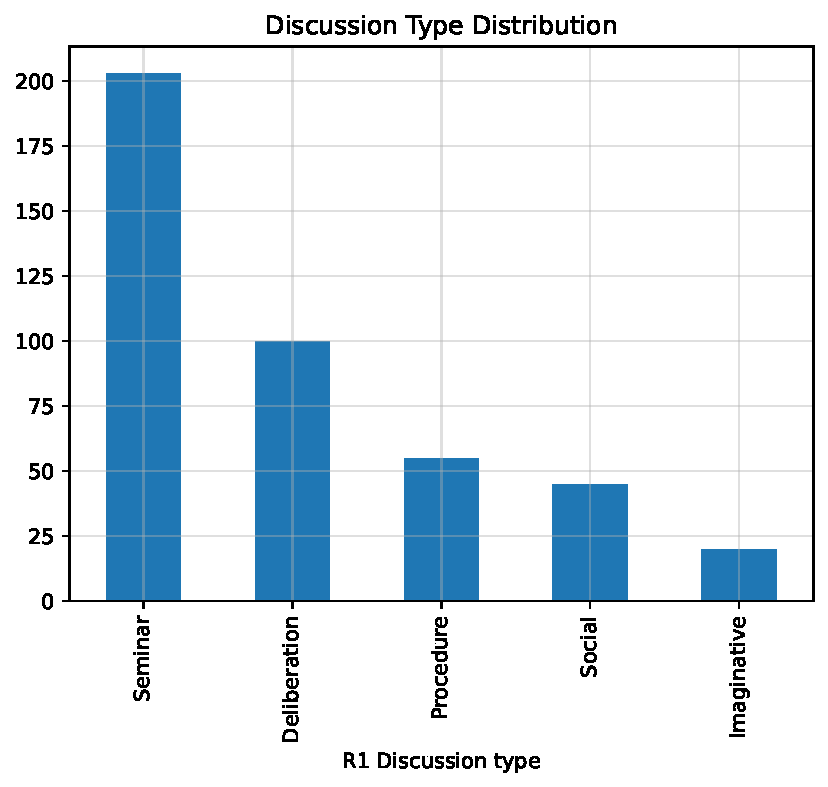
\includegraphics[scale=0.5]{fig/discussion_type_distribution.pdf}
	\caption{Distribution of different discussion types. We can see that 'Seminar' is the predominant type, which is expected from the definition and the type of discourse. The least common type is "Imaginative" which "places the learner in the discussion as an active participant".  }
	\label{fig:distr}
\end{figure}


\iffalse
// UNCOMMENT IF NEEDED //
Additionally, we can analyze the \textit{Pivot} column, which denotes messages that altered the course of discussion, with the formal definition being \textit{The posting establishes or changes the procedural direction of the discussion}. This is evident in Figure \ref{fig:pivot_graph}, where the \textit{Seminar} node occupies the central position with the highest number of connections, aligning with the prevalence of Seminar-type discussions. Outgoing connections are depicted with green arrows, indicating that most pivots originate from \textit{Seminar} and transition into \textit{Deliberation} discussions, and vice versa. This pattern aligns with the definition of \textit{Deliberation} as \textit{Turns related to decision-making about the content}, which often follows or precedes discussions about the story in the \textit{Seminar} type.
 
\begin{figure}[ht!]\centering
	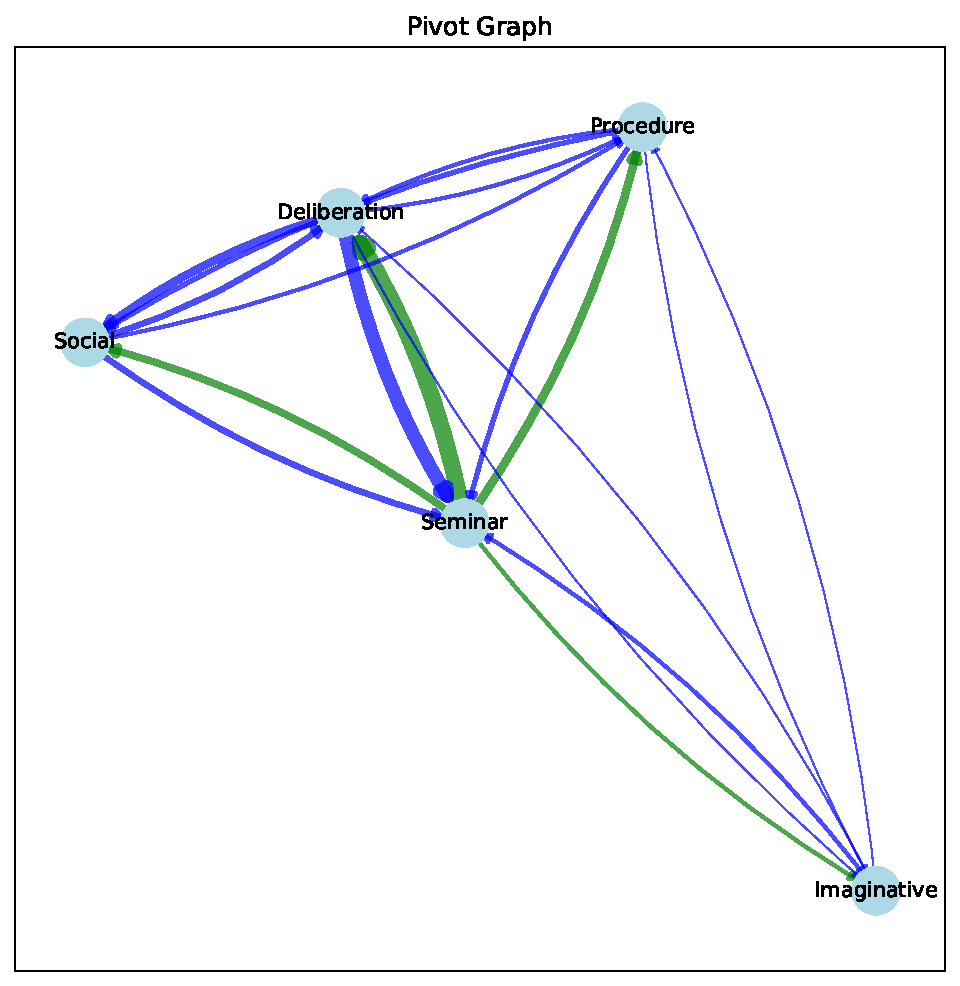
\includegraphics[scale=0.3]{fig/pivot_graph.pdf}
	\caption{The graphical representation illustrates various pivot transitions, with nodes representing different discussion types and lines indicating transitions between them. The width of the lines corresponds to the frequency of specific transitions, while the direction indicates the sequence of occurrences. Notably, thick lines between \textit{Deliberation} and \textit{Seminar} highlight frequent transitions between these two discussion types.}
	\label{fig:pivot_graph}
\end{figure}
\fi


%------------------------------------------------

\section*{Methods}

For the initial phase of our project, we addressed the classification challenge. We chose to utilize the \textit{R2DiscussionType} column as it consistently defines the decision task and serves as the primary class for classification by test subjects. As a benchmark, we employed a pre-trained BERT model (\textit{bert-base-cased}) to classify Discussion types within our dataset. Implementation was carried out using the PyTorch library in Python, which gave us access to Trainer API that we used to fine-tune the pre-trained BERT model. Baseline BERT model was trained with 3 epochs, utilizing a batch size of 8, and employing the standard learning rate of $2 \times 10^{-5}$.

We divided our dataset into three parts: train, test and validation. In the training dataset we have 427 samples or $70\%$ of the dataset, and the test and validation datasets both have 92 samples or $15\%$ of the dataset each. Due to the class imbalance in our dataset, certain less represented classes have only a few samples in the divided datasets. The test dataset is used as an evaluation dataset during the training phase, and we use the validation dataset as a final score of the model.

Using the Trainer API, we could also fine-tune the BERT model by increasing number of epochs. To setup optimizers, we used Adam optimizer by PyTorch and tested a scheduler with implemented \textit{ReduceLROnPlateau}, to reduce learning rate when a metric stops improving.

We also tried using DistilBERT\cite{sanh2020distilbert}, which is a lightweight BERT model fine-tuned for text classification.

Our current plan of work contains several approaches: 
\begin{itemize}[noitemsep]
    \item Implement a different LLM, which will classify discussion types and try to explain how the model made the decision.
    \item Try to use prompt engineering.
    \item Combine two or more models (ensemble learning).
    \item Further exploration of the dataset, possibly filtering out "bad" samples. 
    \item Fine-tune the large BERT model. 
\end{itemize}

We plan to evaluate all our models on a separate discourse dataset, created in a similar research with test subjects being high school students.

%% Prompting
In our exploration of advanced NLP techniques for text categorization, we implemented various methodologies centered around the LLAMA model \cite{decapoda-research-llama-7B-hf} and prompt engineering, aiming to enhance the model's ability to perform few-shot prompting. In order to choose relevant prompts, we experimented with BERT embeddings followed by K-means and hierarchical clustering techniques, which initially did not meet the expected clarity in categorization. Most of the relevant examples chosen by these algorithms were short statements without enough context. Subsequently, we shifted our strategy to use TF-IDF vectorization instead of BERT embeddings. This approach was taken to retain more textual context. However, it didn't prove to be essentially effective in clustering and categorization. The primary limitation we encountered comes from the dataset's composition—specifically, its imbalance and the prevalence of context-poor texts for some categories significantly impacted the LLAMA model's ability to distinguish between categories accurately. Additionally, the names of the categories were also quite abstract for the model to extract features for categorization. This experiment highlighted the critical relationship between dataset quality and the performance of machine learning models in text-based categorization tasks. 

%------------------------------------------------

\section*{Results}
For evaluating our BERT models, we will use accuracy as an evaluation metric to determine how well it is performing. 

\begin{table}[h!]
\begin{adjustbox}{width=\columnwidth,center}
\begin{tabular}{lllll}
Model               & Epochs & Batch size & Test accuracy & Validation accuracy \\
bert-base-cased     & 3      & 4          & 0.728         & 0.652               \\
bert-base-cased     & 3      & 8          & 0.75          & 0.685               \\
bert-base-cased     & 10     & 8          & 0.77          & 0.696               \\
distil-base-uncased & 10     & 8          & 0.728         & 0.641               \\
distil-base-uncased & 50     & 16         & 0.77          & 0.641             \\
bert-large-uncased & 10     & 8         & 0.72     
& 0.72 \\
bert-large-uncased & 20     & 16         & 0.75        
& 0.72
\end{tabular}
\end{adjustbox}
\end{table}

Currently our best performing model is the large BERT model (\textit{bert-large-uncased}), which has the best accuracy score on the validation dataset. The accuracy is greatly affected by the batch size and the number of epochs in which the model was trained.
%------------------------------------------------

\section*{Discussion}



%------------------------------------------------

\section*{Acknowledgments}

%----------------------------------------------------------------------------------------
%	REFERENCE LIST
%----------------------------------------------------------------------------------------
\bibliographystyle{unsrt}
\bibliography{report}


\end{document}